\documentclass{article}
\usepackage[utf8]{inputenc}
\usepackage{graphicx}
\usepackage{float}
\usepackage{xcolor}
\usepackage{listings}
\lstset{
  language=Python,
  basicstyle=\ttfamily\small,
  keywordstyle=\color{blue},
  stringstyle=\color{green},
  commentstyle=\color{red},
  extendedchars=true,
  showspaces=false,
  showstringspaces=false,
  numbers=left,
  numberstyle=\tiny,
  breaklines=true,
  backgroundcolor=\color{green!10},
  breakautoindent=true,
  captionpos=b,
  xleftmargin=0pt,
}

\title{tratamento de imagens}
\author{michelvictor }
\date{May 2019}

\usepackage{natbib}
\usepackage{graphicx}

\begin{document}

\maketitle

\section{Base Ambrapa}
 PDDB possui 2326 imagens de 171 doenças e outras desordens acometendo 21 espécies de plantas \citep{Embrapa}. Apesar de sua significância, PDDB não possui representatividade suficiente para permitir o uso de técnicas como “Deep  Learning”.
 Então foi usado a base XDB, que foi criada a partir da PDDB, seguidos alguns critérios \citep{Embrapa}.   Como  resultado,  esta base de imagens expandida (XDB) atualmente contém 46.513 imagens \citep{Embrapa}.
 

\section{Tratamento da base XDB (Cropped)}
Para agilizar o processo foi criado um script para automatizar o processo de tratamento da base. O trateamento da imagens possui dois processamento principais, o primeiro é validar a imagem, caso em que ela não possuir tamanho suficiente para ser usada, segundo redimensionar todas as imagens para uma mesma dimensão.

Para rodar o script\cite{github} é necessário adotar um arquitetura de pastas

\subsection{Validação de Imagem}
Um dos problemas da base XDB é que ela possui imagens muito pequenas, sem nenhuma representatividade Figura \ref{fig:ferr001}. Para resolver esse problema foi implementado uma um filtragem:

\begin{lstlisting}
# Funcao de validacao
# num_px e num_py, sao as novas dimensoes da imagem
def validaImagem(imagem:Image, taxaDeDiferenca=None)-> bool:
    width, height = 0, 0
    if taxaDeDiferenca:
        width, height = (taxaDeDiferenca * num_px, taxaDeDiferenca * num_py)
    if imagem.size[1] >= (num_px - width) or imagem.size[0] >= (num_py - height):
        return True
    return False
\end{lstlisting}
Considerando \textit{taxaDeDiferenca=None}, o que estar sendo feito na \textbf{linha 9} é uma verificação simples entre o tamanho da imagem com o novo tamanho que ela terá (num\_px, num\_py), se a dimensão da imagem (tupla \textit{imagem.size)} for menor, a mesma é descartada. Caso a função receba \textit{taxaDeDiferenca}, que é um valor em porcentagem, imagens com o tamanho menor que num\_px e num\_py, podem ser usado, caso sejam maior que a diferença entre a porcentagem (\textit{taxaDeDiferenca}) em relação a num\_px e num\_py com (num\_px, num\_py)


\begin{figure}[ht!]
\centering
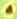
\includegraphics[scale=1]{img/ferr001.jpg}
\caption{17x19 pixels}
\label{fig:ferr001}
\end{figure}

\subsection{Redimensionamento das Imagens}

O Redimensionamento das imagens é bem simples, o segundo \textit{for} serve para abrir cada imagem de uma determinada classe, e em seguida na \textbf{linha 4} a chamada do função de validação, caso em que a imagem não esteja  (\textit{False}) adequada, pula para próxima imagem \textbf{linha 7 e 8}, e no caso contrario (\textit{True}), a imagem vai ser redimensionada e em seguida salva.
\begin{lstlisting}
for ... # for para cada classe/pasta
    for pathImg in imagens:
        image = Image.open(pathImg)
        if validaImagem(image, TAXA_DIFERENCA):
            newImage = image.resize((num_px, num_py))
            newImage.save(NEW_BASE + '/'+ labels[count] +'- '+ str(count)+'/'+str(countImg)+EXTESAO_IMG )
        else:
            continue
\end{lstlisting}

O resultado para uma imagem é mostrado nas Figuras \ref{fig:antes} e \ref{fig:depois}

\begin{figure}[ht!]
\centering
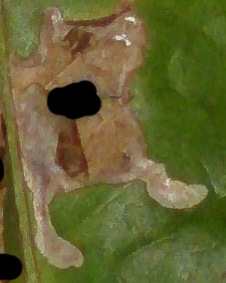
\includegraphics[scale=0.8]{img/antes.jpg}
\caption{Antes do processamento}
\label{fig:antes}
\end{figure}

\begin{figure}[ht!]
\centering
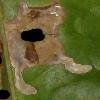
\includegraphics[scale=1]{img/depois.jpg}
\caption{Depois do processamento}
\label{fig:depois}
\end{figure}


\bibliographystyle{plain}
\bibliography{references}
\end{document}
